\chapter{Analysis Validation}
\label{ch:appendix_validation}

In this appendix studies are performed to validate that the analysis framework is functioning correctly and that there are no significant biases in the cross-section results.
In Chapter~\ref{ch:extraction} the default \g configuration was used to extract the cross section. This simulation is used for the estimation of the efficiency and some of the backgrounds. Here, the alternative \g configuration is used (described in Section~\ref{sec:simulation}) to check that the same result (within cross section modelling systematic uncertainties) is obtained.
The default data extract cross section from Eq.~\ref{eq:data_xsec} was
\begin{equation}
\sigma = 0.693 \pm 0.010 \, (\text{stat.}) \times 10^{-38} \, \text{cm}^2.
\end{equation}
Using the alternative \g configuration the cross section is calculated as
\begin{equation}
\sigma^\text{alt.} = 0.714 \pm 0.010 \, \text{(stat)} \times 10^{-38} \,\text{cm}^2.
\end{equation}
The systematic uncertainty due to cross section modelling amount to (see Table~\ref{tab:all_syst}) 0.025 $\times 10^{-38} \,\text{cm}^2$ and covers the value of the cross section extracted with the alternative model set in less than $1\sigma$ range:
\begin{equation}
\text{Number of STD } \sigma \text{ differs from } \sigma^\text{alt.} = \frac{0.714-0.693}{0.025} = 0.84.
\end{equation} 

The comparison is also done for the two single differential cross sections (similar results are obtained with the double-differential cross section), as shown in Figure \ref{fig:xsec_tune1_tune3}. The plots show the data cross section extracted using the ``\tuneone'' configuration in black, and using the ``\tunethree'' configuration in red. Also here, the data cross section doesn't change drastically going from one model set to another, confirming that the cross section extraction is robust. The vertical bars show the systematic uncertainties on the default extracted cross section, only from cross-section modelling. This is done in order to show that the error bars cover the difference between the two cross sections in every bin.

\begin{figure}[]
%\begin{adjustwidth}{-1cm}{-1cm}
\centering
\subfloat[][]
   {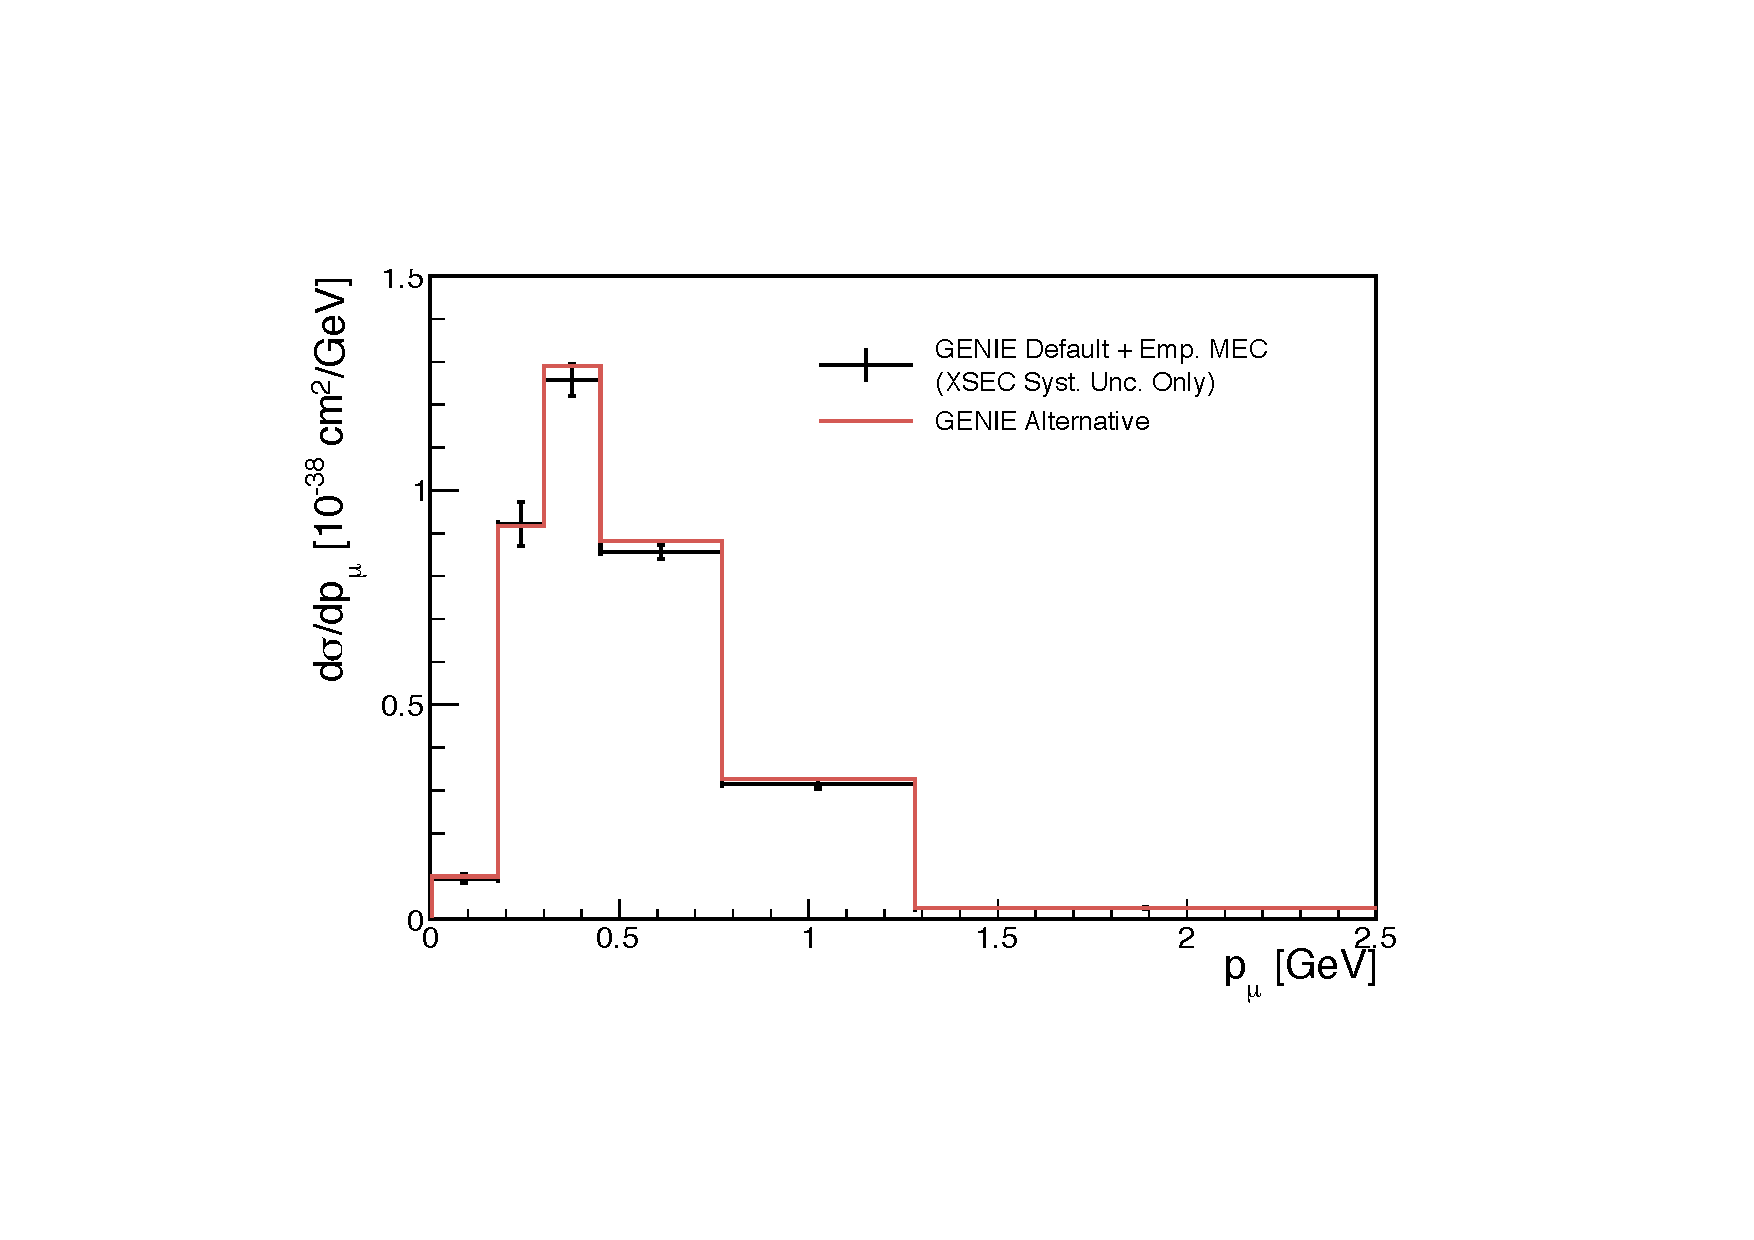
\includegraphics[width=.5\textwidth]{images/XSecTune1Tune3Comparison/xsec_tune1_tune3_mumom_2}
   \label{fig:xsec_tune1_tune3_mumom}} 
\subfloat[][]
   {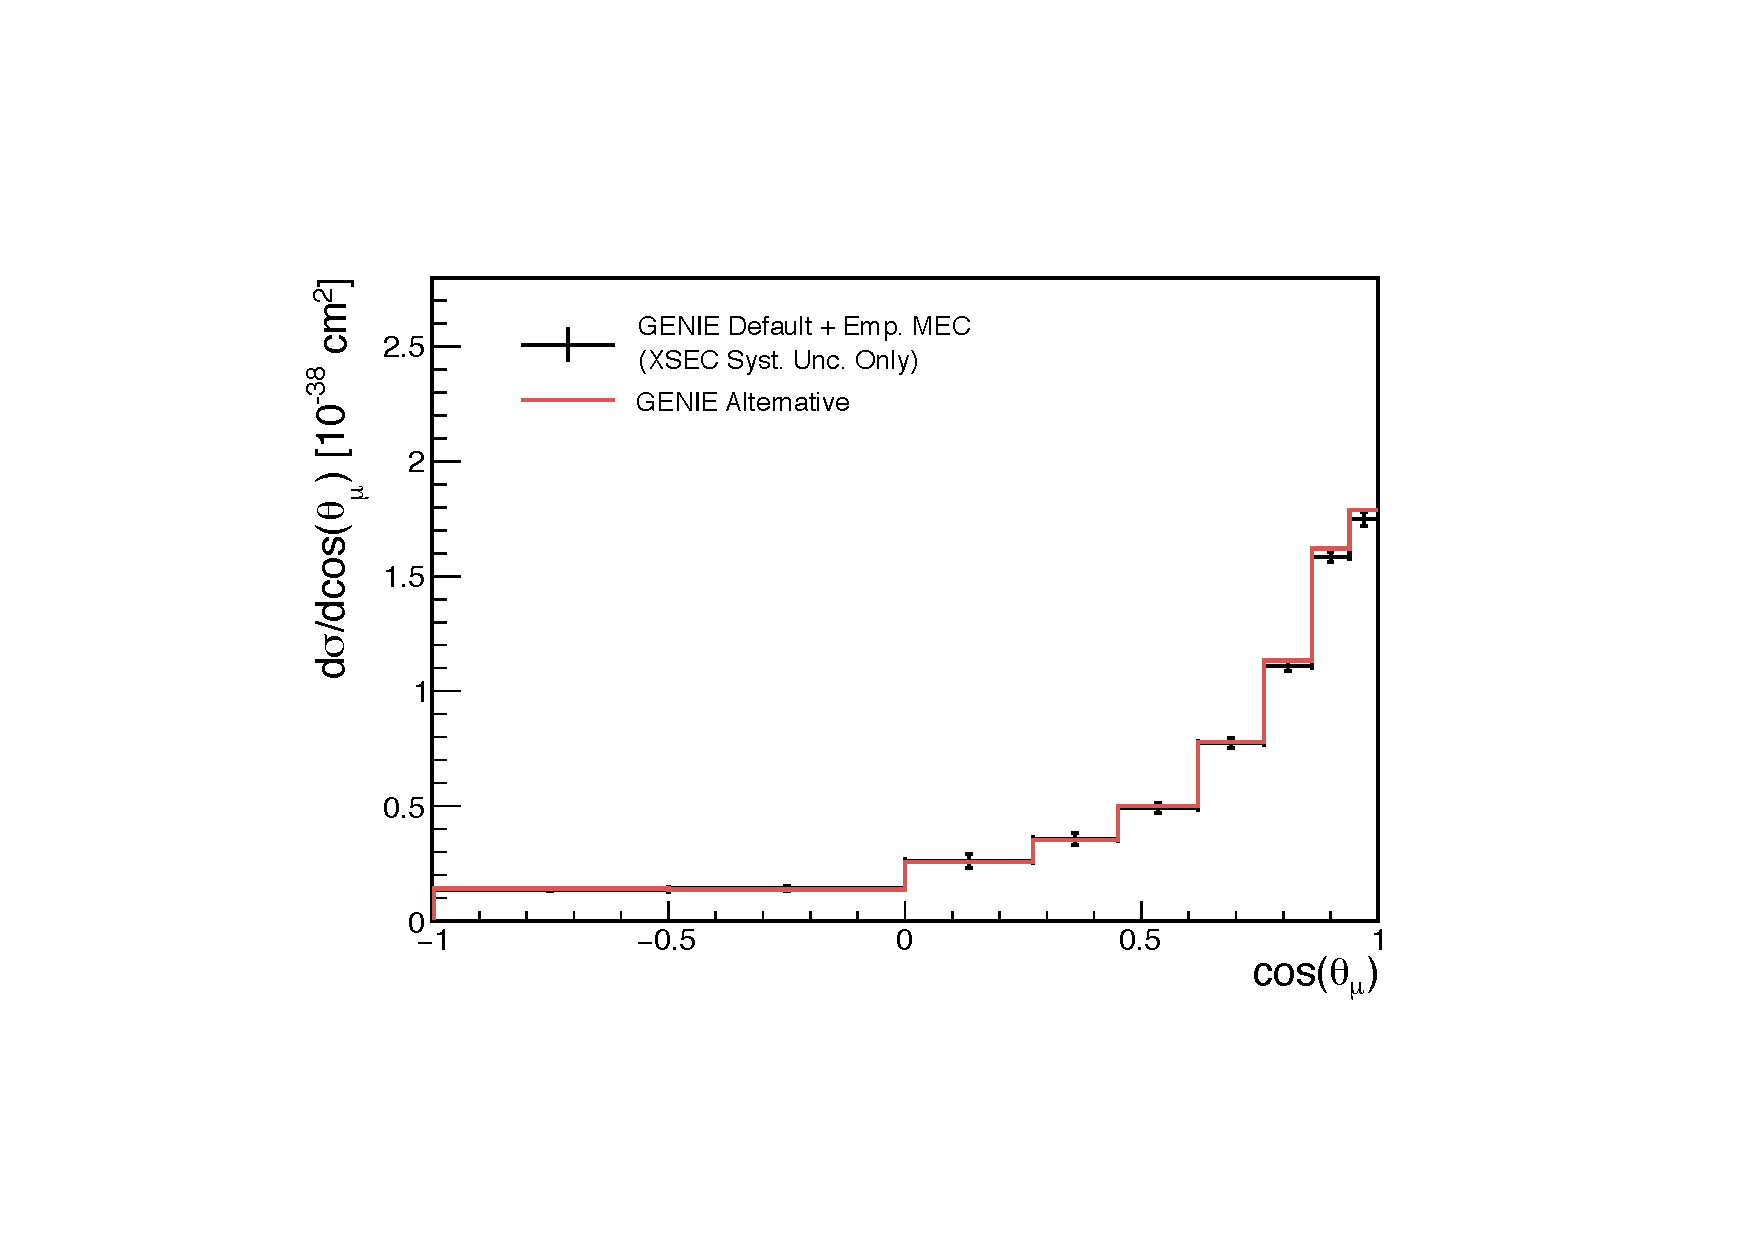
\includegraphics[width=.5\textwidth]{images/XSecTune1Tune3Comparison/xsec_tune1_tune3_muangle_2}
   \label{fig:xsec_tune1_tune3_muangle}} \\
\caption[Single-Differential Cross Section Extracted with Different Simulations]{Single-differential cross section in $p_\mu$~\protect\subref{fig:xsec_tune1_tune3_mumom} and $\cos\theta_\mu$~\protect\subref{fig:xsec_tune1_tune3_muangle} extracted using two different simulations for background and efficiency estimations. The black points shows the data cross section extracted using the ``\tuneone'' simulation (default MicroBooNE simulation). The error bars show systematic uncertainties from cross section modelling only. The red shows the data cross section extracted using the ``\tunethree'' simulation.}
\label{fig:xsec_tune1_tune3}
%\end{adjustwidth}
\end{figure}


Moreover, a fake data test is used to validate the analysis framework. For this test, the \g alternative  \acrshort{mc} is used as fake data. This is shown in Figure~\ref{fig:xsec_fakedata} for the two single -differential cross sections (similar results are obtained with the double-differential cross section). The green is pure \acrshort{mc} from \g default, while the black data points show the fake data (\g alternative) extracted cross section. 
To ensure that the cross section extraction is done properly, the \g alternative cross section, simulated in true momentum and angle bins, has been smeared using the smearing matrices from Figure~\ref{fig:trkmom_migration_matrix_2d} and~\ref{fig:trkangle_migration_matrix_2d}, and compared to the black data point. This is shown with the yellow line in Figure~\ref{fig:xsec_fakedata}. The fake data points match the true prediction within the cross section modelling systematic uncertainties (vertical bars) which validates the cross section extraction.

\begin{figure}[]
%\begin{adjustwidth}{-1cm}{-1cm}
\centering
\subfloat[][]
   {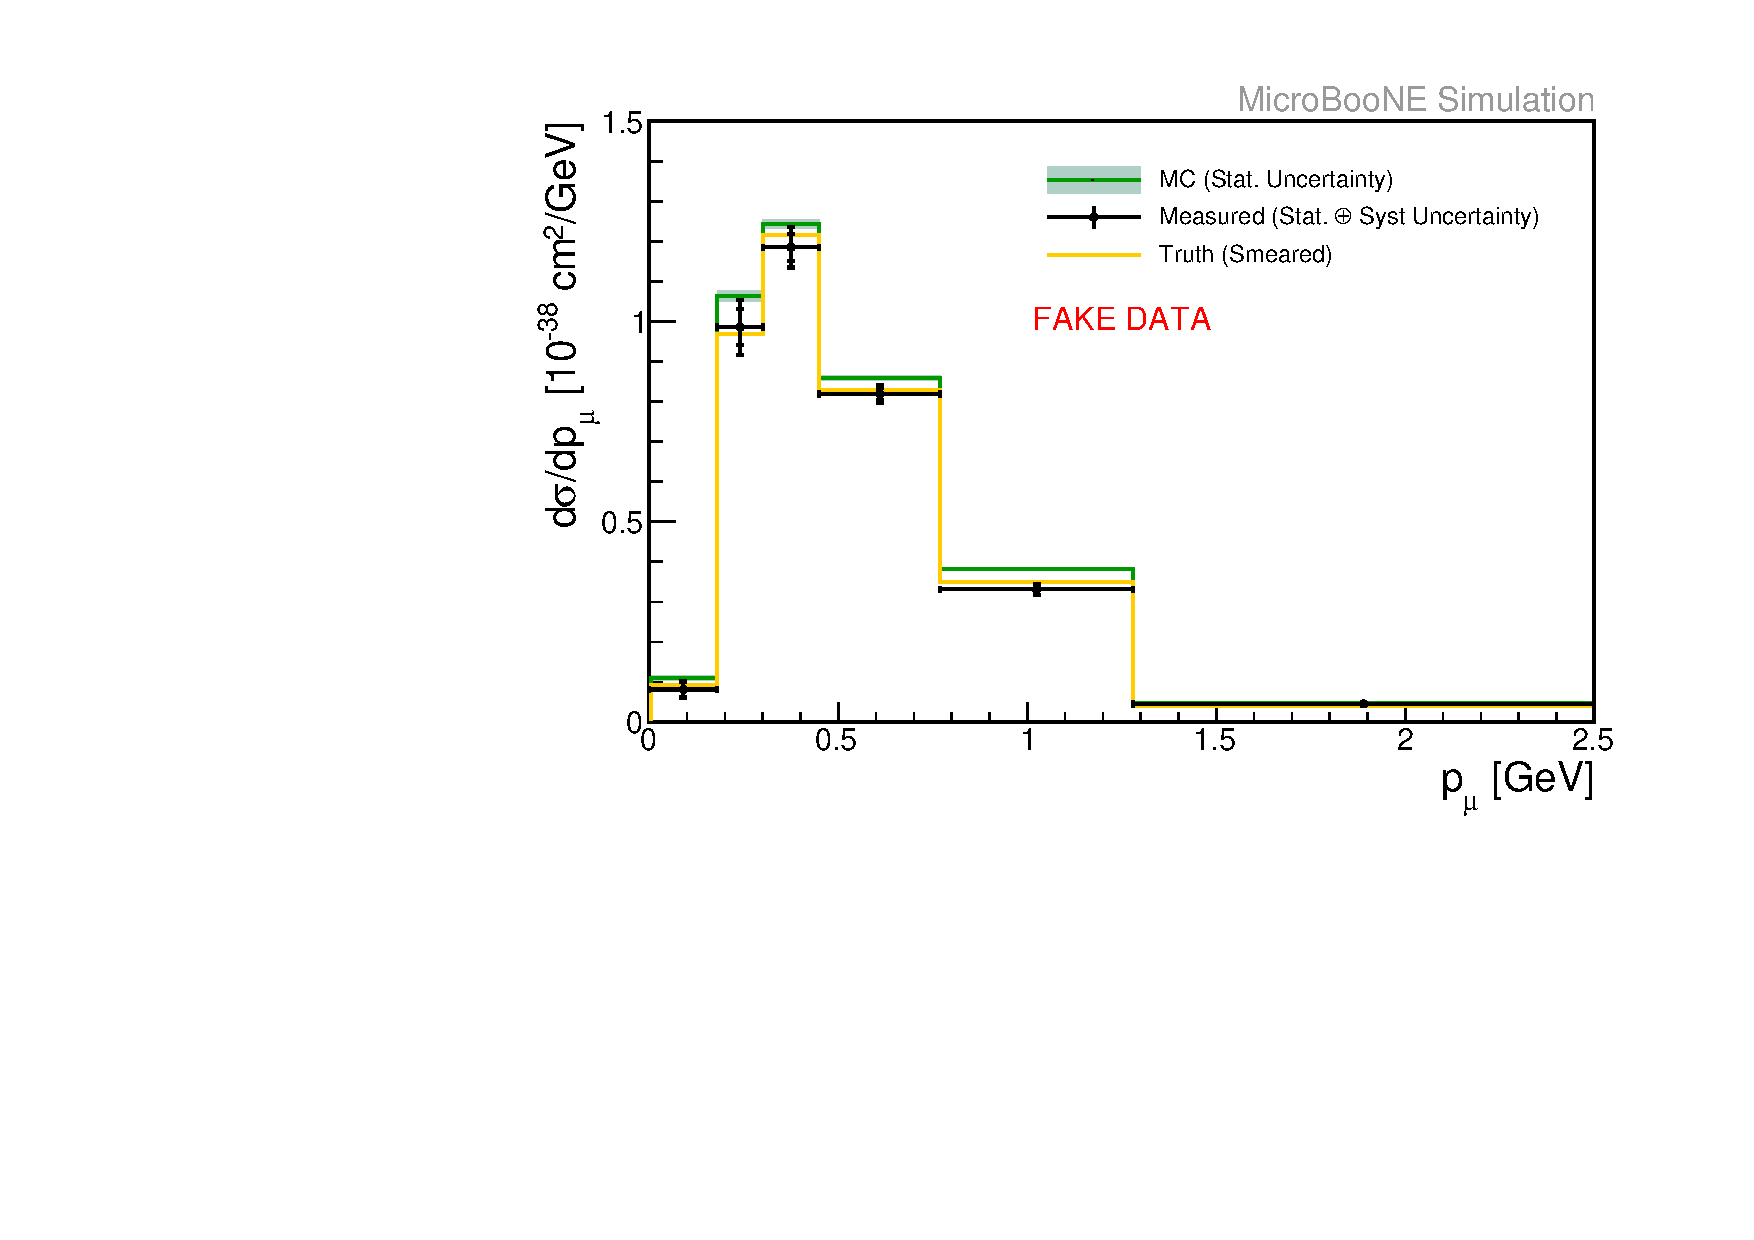
\includegraphics[width=.5\textwidth]{images/XSecFakeData/trkmom_xsec_fakedata}
   \label{fig:trkmom_xsec_fakedata}}
\subfloat[][]
   {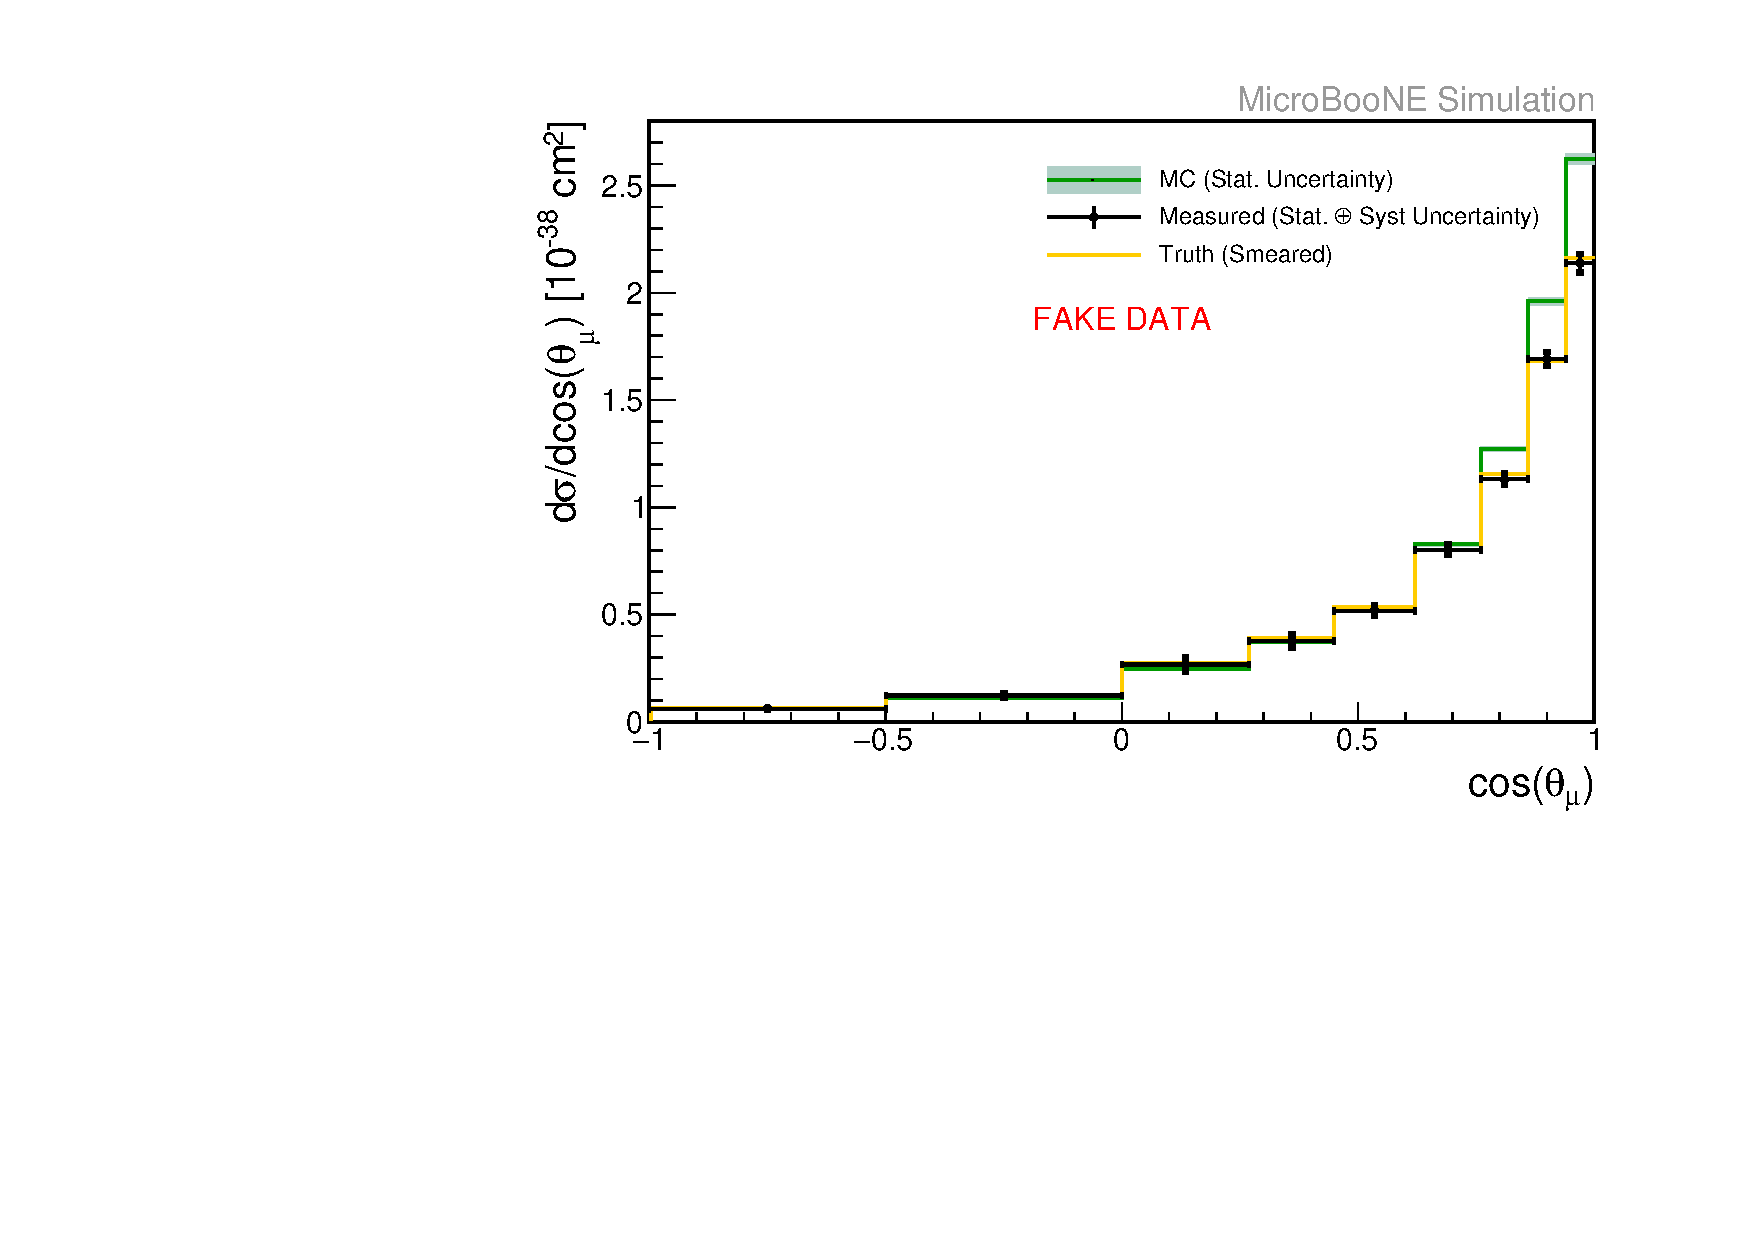
\includegraphics[width=.5\textwidth]{images/XSecFakeData/trkcostheta_xsec_fakedata}
   \label{fig:trkcostheta_xsec_fakedata}} \\
\caption[Single-Differential Cross Section Extracted with Fake Data]{Single-differential cross section in $p_\mu$~\protect\subref{fig:trkmom_xsec_fakedata} and $\cos\theta_\mu$~\protect\subref{fig:trkcostheta_xsec_fakedata} extracted using using a sample of fake data from an alternative simulation. The green shows the \acrshort{mc} only extracted cross section from the ``\tuneone'' simulation (default MicroBooNE simulation)s. The black points are a fake data simulation. They are obtained from a sample generated with the ``\tunethree'' model configuration. The orange shows the truth \g cross section from ``\tunethree'', smeared using the migration matrix from Figure~\ref{fig:trkmom_migration_matrix_2d} and~\ref{fig:trkangle_migration_matrix_2d}. Only systematic uncertainties from cross section modelling are included here (vertical bars).}
\label{fig:xsec_fakedata}
%\end{adjustwidth}
\end{figure}











